\documentclass[lettersize,journal]{IEEEtran}
\usepackage{amsmath,amsfonts}
\usepackage{algorithmic}
\usepackage{algorithm}
\usepackage{array}
\usepackage[caption=false,font=normalsize,labelfont=sf,textfont=sf]{subfig}
\usepackage{textcomp}
\usepackage{stfloats}
\usepackage{url}
\usepackage{verbatim}
\usepackage{graphicx}
\usepackage{cite}
\usepackage[hypcap=false]{caption}
\usepackage{float}

% Set path for images
\graphicspath{ {./images/} }

\newenvironment{Figure}
    {\par\medskip\noindent\minipage{\linewidth}}
    {\endminipage\par\medskip}


\begin{document}

\title{An Explainable Machine Learning Approach to Antenna Design}

\author{Tyler Carr \\ carrt12@my.erau.edu \\ Embry-Riddle Aeronautical University \\ Daytona Beach, FL}

\maketitle

\begin{abstract}
Antenna design processes require extensive simulation tasks that are resource and time intensive, which are prone to interruptions. Design equations are only available for a predefined and limited set of antenna geometries. By applying a machine learning algorithm to data that has already been generated from simulations of an antenna, performance metrics can be predicted significantly quicker than running full simulations. Insights about which geometric parameter had the most significant impact on the prediction can be drawn from the model and included in the output. Additionally, the model can be reversed so that for a particular form of antenna, an optimal geometry can be produced that will result in a specified performance and frequency range. 
\end{abstract}

\section{Introduction}
Antenna designs require simulation in order to determine the performance of the antenna. Ansys High Frequency Simulation Software (HFSS) is an electromagnetic simulation software which is used to design and simulate antennas between a range of frequencies. When designing the antenna, details such as dimensions of the antenna geometry, materials used for the antenna, and frequency are specified~\cite{Maxworth_2022}. Simulations are then run. These simulations produce S11 values, which are the reflection coefficients. These represent the amount of power that is reflected from the antenna, and is measured in decibels. This value is always negative, and a lower value means the antenna is performing more efficiently. Ideally, this value is below -10dB~\cite{Bevelacqua_2015}.


\subsection{Dataset}
Two datasets were used to train and test the machine learning models. Both datasets were generated from a parametric sweep of the antenna. The two antennas that were used were a patch antenna and a leaky wave antenna. The seven features of the patch antenna dataset contained inset\_dist, L, sub\_thick, W, W0, y0, and Freq, with all measurements being in millimeters except frequency being GHz. The seven features of the leaky wave antenna dataset include Feed\_Gap (mm), Feed\_Inset (cm), Feed\_W (cm), Ground\_gap (mm), Pad\_L (cm), Pad\_W (cm), and Freq (GHz). All of the features except the frequency represent a part of the antenna's geometry. Each of the features were paired with a label, which is a S11 value. 


\subsection{Simulation Issues}
The main issue with running simulations in HFSS is the amount of time that it takes. The matrix operations that are required to run many iterations of simulations to analyze loss can take multiple days to complete~\cite{john_antenna_2009}. Depending on how the simulation is set up, this process could be impacted by power outages or software bugs, resulting in a loss of data and requiring manual intervention to re-run the simulation. 

HFSS works by specifying a range of dimensions and outputting performance metrics, such as S11 values. This is insightful, but there is a degree of trial and error involved in finding an optimal antenna geometry. One would start by specifying what they would think would be the ideal antenna geometry using their own intuition. Based on the results from an initial simulation run, geometry values would be adjusted in an attempt to optimize the geometry.

By using a machine learning algorithm to do the bulk of the investigative work, the amount of simulation iterations that need to be run to optimize an antenna's geometry can be significantly reduced. By training the model on the 405 geometries, frequencies, and S11 values, permutations of more geometries and frequencies can be generated and new S11 values can be predicted. These predictions can be searched, making it easier and quicker to narrow down to a specific area of interest without having to wait for simulations to run.


\subsection{Reversing the Problem}
After training a machine learning model on the dataset, a table is produced with significantly more rows than was started with from the simulated data. Predictions can be searched by specifying the desired S11 value and a range of frequency values that the antenna should operate between. Antenna geometries that match the search are returned, which saves significant time that would be required to set up and perform additional simulations. When seeking an optimal geometry between a certain frequency range, the geometry that results in the S11 with the lowest maximum S11 range would be chosen.


\section{Related Work}
Machine learning topics with antenna design optimizations have been explored before. The algorithm and methods that are chosen ultimately depend on the way that the antenna geometry is expressed. One format that the input data can have is to be in tabular format, where rows represent combinations of geometry measurements and some performance specification, such as S11. For rows of data, algorithms that have been used before can be something like a Artificial Neural Networks, Gaussian Network, or Gaussian Process Regression. The other type of format that the input data can have would be where the geometry is represented with pixels with a matrix of integers each representing a different material being used. This second format is useful for Convolutional Neural Networks and allows for exploring new antenna geometry designs instead of only staying within predefined restrictions.~\cite{wu_machine_2023} 

TODO ADD MORE 


\section{Methodology}
In order to determine the optimal antenna geometry, a machine learning algorithm was employed. This algorithm is trained with a supervised learning method using the parametric sweep dataset for the antenna geometry. Because the data is generated from a parametric sweep, it contains many different combinations of geometries. For the patch antenna, out of the 40,905 rows, there were 405 unique geometries that each had a simulated S11 value for the same frequency range between 4 to 12. In order to generate more data, more values for each geometry feature were inserted between the minimum and maximum of each feature. Generating all the permutations of the geometries and frequencies added up to a total of 9,720 unique geometries, which includes the original 405. The real S11 values are used for the original 405, but predictions are generated for the rest of the geometry and frequency combinations. This new dataset includes a total of 981,720 rows. Similarly, for the leaky wave antenna, there were 21 unique geometries that were used as training data between a frequency range between 2 to 20. There were 555 unique geometries in the end for this antenna design. These generated values for each antenna aided in providing a better guess of an optimal geometry for a specfiied S11 and frequency range, helping optimize the antenna faster. 

\subsection{Analyzing the Data}
In order to determine if a S11 value was predicted accurately, a tolerance was utilized. An exact prediction of an S11 value with high precision is very unlikely, so this tolerance allows for some flexibility. The tolerance is the error that we allow the value to contain, and we consider the prediction accurate if it is within the range specified by the tolerance either above or below the true value. The tolerance is important for an accurate model, and ideally this value should be below one.

A regression algorithm was chosen as the label is numeric. 20\% of the dataset provided by the parametric sweep was reserved for testing and comparing the performance of the models, and the remainding 80\% was used to train the models. Two common metrics to compare algorithm performance in addition to the tolerance mentioned above are the $R^2$ score~\eqref{eq:rsquared} and the RMSE (Root Mean Squared Error)~\eqref{eq:rmse}~\cite{haque_machine_2023,m_el-kenawy_optimized_2022}. 

\begin{figure}[h]
    \begin{equation}
        R^2 = 1 - \frac{\text{SSR}}{\text{SST}}
        \label{eq:rsquared}
    \end{equation}
    \begin{equation}
        {RMSE} = \sqrt(\frac{1}{n} \sum_{i=1}^{n}(y_i - \hat{y}_i)^2)
        \label{eq:rmse}
    \end{equation}
    \caption{Formulas for R-squared and RMSE}
\end{figure}


\subsection{Preprocessing}
Preprocessing is a necessary step with any data being processed through a machine learning algorithm. Only after the data is preprocessed will it yield beneficial results from the algorithm.

The first step was to exclude any data that was considered invalid. Data points with S11 values that are greater than zero are ignored. This should never happen in a real scenario, and if this occurs, it means that there was an error with the calculation. 

The next preprocessing action that was performed was scaling. This process linearly transforms the ranges of the geometry parameters to have the same scale. This is performed so all features are weighted the same and no one feature is artificially weighted more than the others.


\subsection{Comparing Models}
Two different libraries were compared in order to determine the best model for this type of dataset. The first library that was used is TensorFlow, which was used to create a DNN (deep neural network). The performance of the DNN was compared to many of Scikit-learn's regression models.

To keep the comparison between the algorithms fair, all preprocessing steps were performed in the same way when comparing the performance of different libraries and algorithms. When splitting the dataset into training and testing portions, the dataset was split with the same random state, meaning that every model received the same random subset of data for training. Additionally, the models were evaluated in the same way using the same performance metrics between the different libraries. All of the following were performed on the same machine to eliminate the possibility of hardware anomalies. The machine that was used contained a  Intel\textregistered~Core\texttrademark~i9\-10900X CPU @ 3.70GHz and a NVIDIA GeForce RTX 3090 graphics card. 


\subsection{TensorFlow}
TensorFlow was used to create a DNN (deep neural network), which is useful for large datasets. The main benefit of a DNN is that it automatically figures out the most important correlations between features for you. 

The hyperparameters of the DNN were tuned in an attempt to both improve the accuracy and reduce the error rate of the model. This was done by adjusting various hyperparameters of the model, including the number of layers in the network, the rate at which the model learns, andw the unit of each layer, which represents the number of neurons and outputs. This was done using a randomized searching method. In typical grid search hyperparameter tuning, the search space grows too large to be feasibly tested fairly quickly. With the randomized search method, a random subset of hyperparameter combinations can be tested. The most optimal results are not guaranteed, but it can get relatively close~\cite{omalley2019kerastuner}. 


\subsection{Scikit-learn}
Scikit-learn is another popular machine learning library where the typical use case is smaller datasets with feature extraction already having been performed. There are a multitude of regression models provided by Scikit-learn. The models that were analyzed in this test were RandomForestRegressor, GradientBoostingRegressor, AdaBoostRegressor, SVR, CatBoostRegressor, XGBRegressor, and DecisionTreeRegressor.

Similarly to with TensorFlow, a randomized search was used to determine the best hyperparameters for each model's use case. Once the optimization was performed, all of the best models had their performance compared using the same metrics. 

\subsection{Finding Optimal Geometry}
The flowchart in Figure~\ref{data_flow} gives a visual representation of how the data flows through the algorithm. All of the steps up until generating predictions are performed initially for any new antenna configuration that the model hasn't seen yet. The last few steps, starting at filtering rows, are performed every time a new optimal geometry is searched using a specified S11 and frequency range. 

\begin{Figure}
\centering
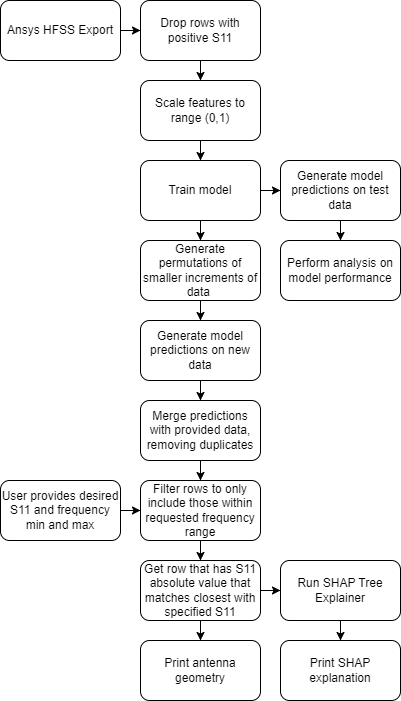
\includegraphics[width=3.0in]{methodology}
\captionof{figure}{Flow of data through the system}
\label{data_flow}
\end{Figure}

A GUI (graphical user interface) was created in order to make the process of filtering optimal geometries more intuitive. The GUI include an input area, where a user can input a desired S11 and frequency range. Once these are entered, all of the permutations are filtered and the best performing optimal geometries are shown. A graph of frequency and predicted S11 is also shown, where each optimal geometry is plotted. The desired S11 and frequency range are also represented on the graph so it's clear what area of the graph is being focused on.


\section{Results}
\subsection{Library and Model Comparison with the Patch Antenna}
The patch antenna was used to test and compare the performance of models from the two different libraries: TensorFlow and Scikit-learn. The best performing model was chosen from each library, and their training time, predicting time, accuracy, and RMSE were compared in order to select the best model.

The Keras Tuner search for optimal hyperparameters of the DNN provided the results in Table~\ref{keras_best_params}. It found that the model performed best with the maximum number of layers out of the testing range, and the optimal learning rate was in the middle of the testing range. This DNN was only able to predict S11 values with an error tolerance of~$\pm$1dB with a 31.75\% accuracy. This low accuracy gives the hint that this might not be the best model for the job.

TODO UPDATE TABLE WITH NEW VALUES and above with new percentage accuracy 

\begin{table}[h]
\caption{Keras Tuner Best Hyperparameters}
\begin{center}
\begin{tabular}{ |c|c|c| }
    \hline
    Hyperparameter Name & Hyperparameter Value \\ 
    \hline
    num\_layers & 4 \\  
    \hline
    units\_0 & 256 \\
    \hline
    units\_1 & 32 \\
    \hline
    units\_2 & 32 \\
    \hline
    units\_3 & 32 \\
    \hline
    learning\_rate & 0.011724 \\
    \hline
\end{tabular}
\end{center}
\label{keras_best_params}
\end{table}

Figure~\ref{dnn_loss_graph} shows how the DNN's loss decreased as the number of epochs increased. The fact that this graph shows both the training and testing decreasing shows that the model is converging. Additionally, the model is not overfitting. 

\begin{Figure}
    \centering
    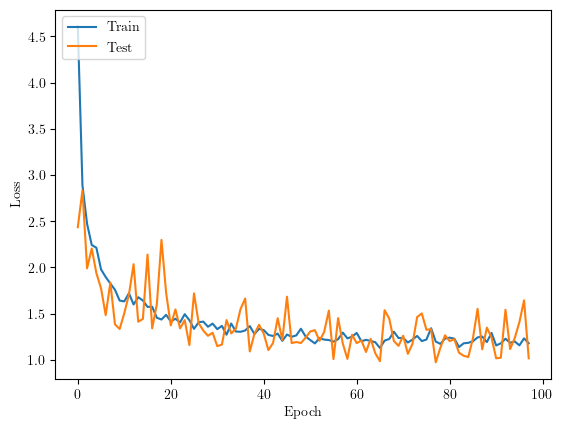
\includegraphics[width=2.5in]{loss}
    \captionof{figure}{DNN Loss Graph}
    \label{dnn_loss_graph}
\end{Figure}

Each of the Scikit-learn regression models performed differently than one another. After performing a randomized search for the best hyperparameters for each type of model, the score of the best configuration of each model was reported alongside the $R^2$ and RMSE scores. Please see Table~\ref{comparing_sklearn} for a summary of the results. The table is sorted by best to worst performance by score, RMSE, and $R^2$. The goal is to have the highest accuracy and the lowest RMSE $R^2$. 

It's clear by looking at the table that RandomForestRegressor is the best performing model. It has the highest accuracy and the lowest RMSE, which proves that its predictions had the least distance from the actual S11 values. When comparing TensorFlow to Scikit-learn, this is the model that will be used. 

\begin{table}[h]
\caption{Scikit\-learn Results}
\begin{center}
\begin{tabular}{ |c|c|c|c| }
    \hline
    Model Type & Accuracy within~$\pm$1dB & RMSE & $R^2$ \\ 
    \hline
    RandomForestRegressor & 0.9301 & 0.7652 & 0.9620 \\
    \hline  
    DecisionTreeRegressor & 0.9080 & 1.0764 & 0.9248 \\  
    \hline
    GradientBoostingRegressor & 0.9012 & 0.9950 & 0.9357 \\
    \hline
    CatBoostRegressor & 0.8969 & 0.9949 & 0.9358 \\    
    \hline
    XGBRegressor & 0.8942 & 1.0467 & 0.9289 \\  
    \hline
    AdaBoostRegressor & 0.8526 & 1.1924 & 0.9077 \\  
    \hline
    SVR & 0.6717 & 2.7252 & 0.5180 \\  
    \hline
\end{tabular}
\end{center}
\label{comparing_sklearn}
\end{table}

When comparing the TensorFlow and Scikit-learn libraries, the same random state was used when splitting the data into training and testing portions. This ensures that each library is given a fair chance with the same set of data and the data isn't being swayed unintentionally. The TensorFlow model had 500 epochs, but only used 44 of them due to the early stopping criteria that was set. 

TODO FIX NUMBERS BELOW

It's clear from the Table~\ref{comparing_libraries} that Scikit-learn is the best choice of library for this problem. The Scikit-learn model performed with 28.42\% better accuracy when predicting values with a tolerance of~$\pm$1dB. It trains and predicts significantly faster, and it has a lower RMSE.

\begin{table}[h]
\caption{Comparing Libraries}
\begin{center}
\begin{tabular}{ |c|c|c| }
    \hline
    Model Type & TensorFlow & Scikit-learn \\ 
    \hline
    Training Time (s) & 67.0 & 32.7 \\  
    \hline
    Predicting Time (s) & 0.327 & 2.17 \\
    \hline
    S11 Accuracy within~$\pm$1dB & 0.7757 & 0.9301 \\
    \hline
    RMSE & 2.2026 & 0.7652 \\
    \hline
\end{tabular}
\end{center}
\label{comparing_libraries}
\end{table}

Figure~\ref{histogram_of_error_patch} shows how the Sklearn model had lower error between the predicted S11 values and the actual S11 values than the TensorFlow model for the patch antenna. The TensorFlow model tended to make predictions that were lower than the actual values. Additionally, Figure~\ref{actual_vs_predicted_s11_patch} demonstrates how the S11 predictions were closer to the actual values, which is depicted by the diagonal line, for the Sklearn model. The TensorFlow model had trouble predicting thet outliers. 

\begin{Figure}
    \centering
    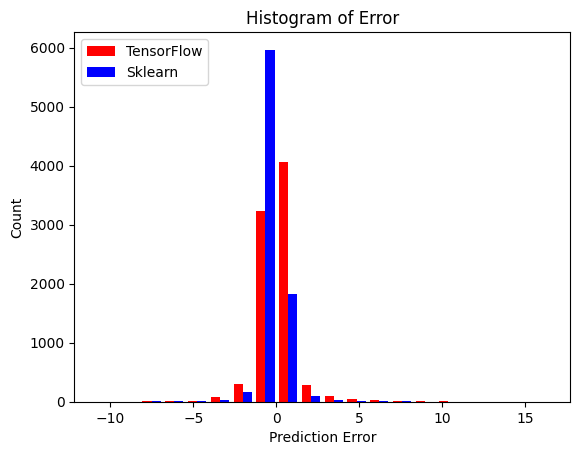
\includegraphics[width=2.5in]{histogram_patch}
    \captionof{figure}{Histogram of Error for Patch Antenna}
    \label{histogram_of_error_patch}
\end{Figure}

\begin{Figure}
    \centering
    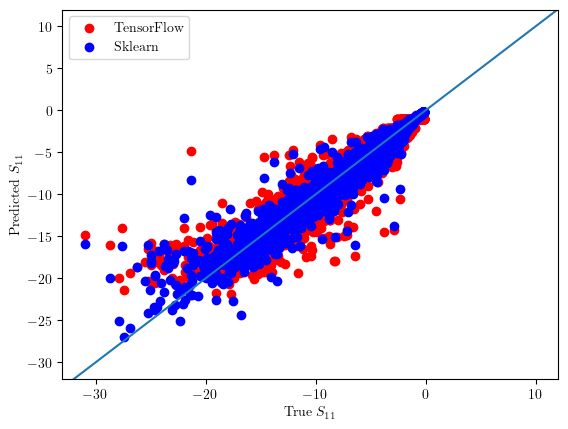
\includegraphics[width=2.5in]{actual_vs_predicted_s11_patch}
    \captionof{figure}{Actual vs Predicted S11 for Patch Antenna}
    \label{actual_vs_predicted_s11_patch}
\end{Figure}

Figures~\ref{histogram_of_error_leaky_wave} and~\ref{actual_vs_predicted_s11_leaky_wave} show how the results for the leaky wave antenna are similar to those of the patch antenna. The leaky wave antenna was trained on significantly fewer geometries, and both figures show how the models were predicting with less accuracy for both Scikit-learn and Tensorflow. However, this does prove that Scikit-learn performed better for both antenna configurations.

\begin{Figure}
    \centering
    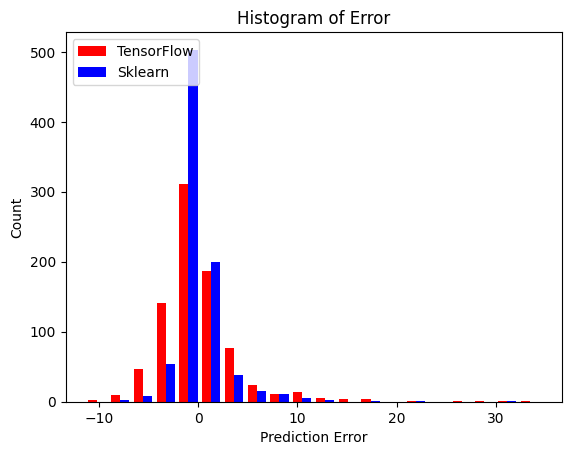
\includegraphics[width=2.5in]{histogram_leaky_wave}
    \captionof{figure}{Histogram of Error for Leaky Wave Antenna}
    \label{histogram_of_error_leaky_wave}
\end{Figure}

\begin{Figure}
    \centering
    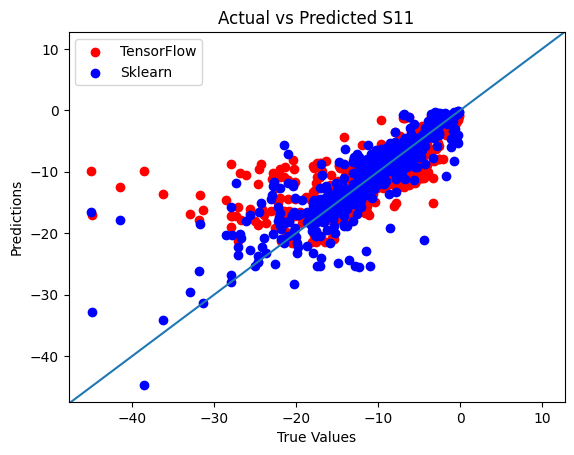
\includegraphics[width=2.5in]{actual_vs_predicted_s11_leaky_wave}
    \captionof{figure}{Actual vs Predicted S11 for Leaky Wave Antenna}
    \label{actual_vs_predicted_s11_leaky_wave}
\end{Figure}

\subsection{Testing with Completely Unseen Data}
The chosen model was given a set of 3 geometries that had never been seen before by either the training set or testing set. They 

TODO FIX ME 

\subsection{Finding Optimal Geometry}
TODO talk about gui here 

TODO replace image with something more high quality, find better example 

\begin{Figure}
    \centering
    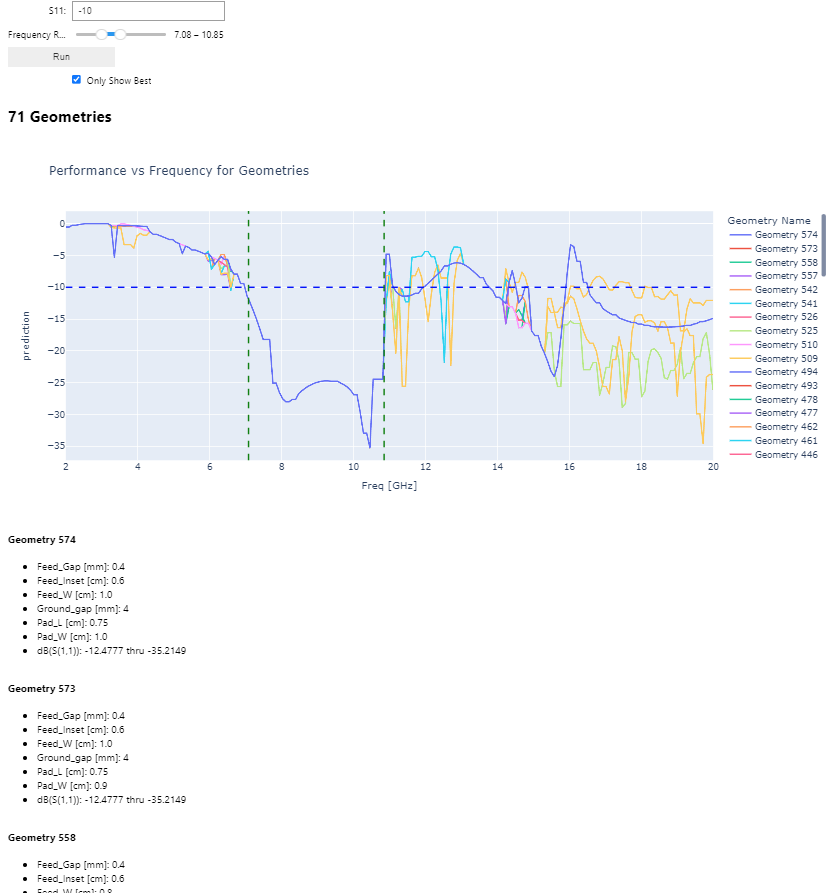
\includegraphics[width=2.5in]{gui}
    \captionof{figure}{Actual vs Predicted S11}
    \label{gui}
\end{Figure}


\section{Conclusion}

TODO CITE CAMERON for data
TODO cite TensorFlow


\bibliographystyle{IEEEtran}
\bibliography{refs}

\vfill

\end{document}